\documentclass[8pt, a4paper, oneside, final]{scrartcl}
\usepackage{soul}
\usepackage{scrpage2}
\usepackage{titlesec}
\usepackage{lipsum}
\usepackage[usenames, dvipsnames]{color}
\usepackage{amsfonts,graphicx}
%\usepackage[pdfstartview=FitH,urlcolor=blue,colorlinks=true,bookmarks=true]{hyperref}
\usepackage[pdfstartview=FitH,pdfcreator={Drasko DRASKOVIC}]{hyperref}
\usepackage{marvosym}
\usepackage{tabularx,colortbl}
\usepackage{amssymb}
\usepackage{fontawesome}
\usepackage{dashrule}
\usepackage[svgnames]{xcolor}
\usepackage{graphicx}
\usepackage[margin=0.1\textwidth]{geometry}
\usepackage{wrapfig}

\pagestyle{plain}   % do page numbering ('empty' turns off)
\frenchspacing      % no aditional spaces after periods

\titleformat{\section}         % Customise the \section command
  {\Large\scshape\raggedright} % Make the \section headers large (\Large),
                               % small capitals (\scshape) and left aligned (\raggedright)
  {}{0em}                      % Can be used to give a prefix to all sections, like 'Section ...'
  {}                           % Can be used to insert code before the heading
  [\titlerule]                 % Inserts a horizontal line after the heading

\titleformat{\subsection}
  {\large\scshape\raggedright}
  {}{0em}
  {}



\begin{document}

  \begin{tabular}{@{}m{0.15\linewidth}l}

    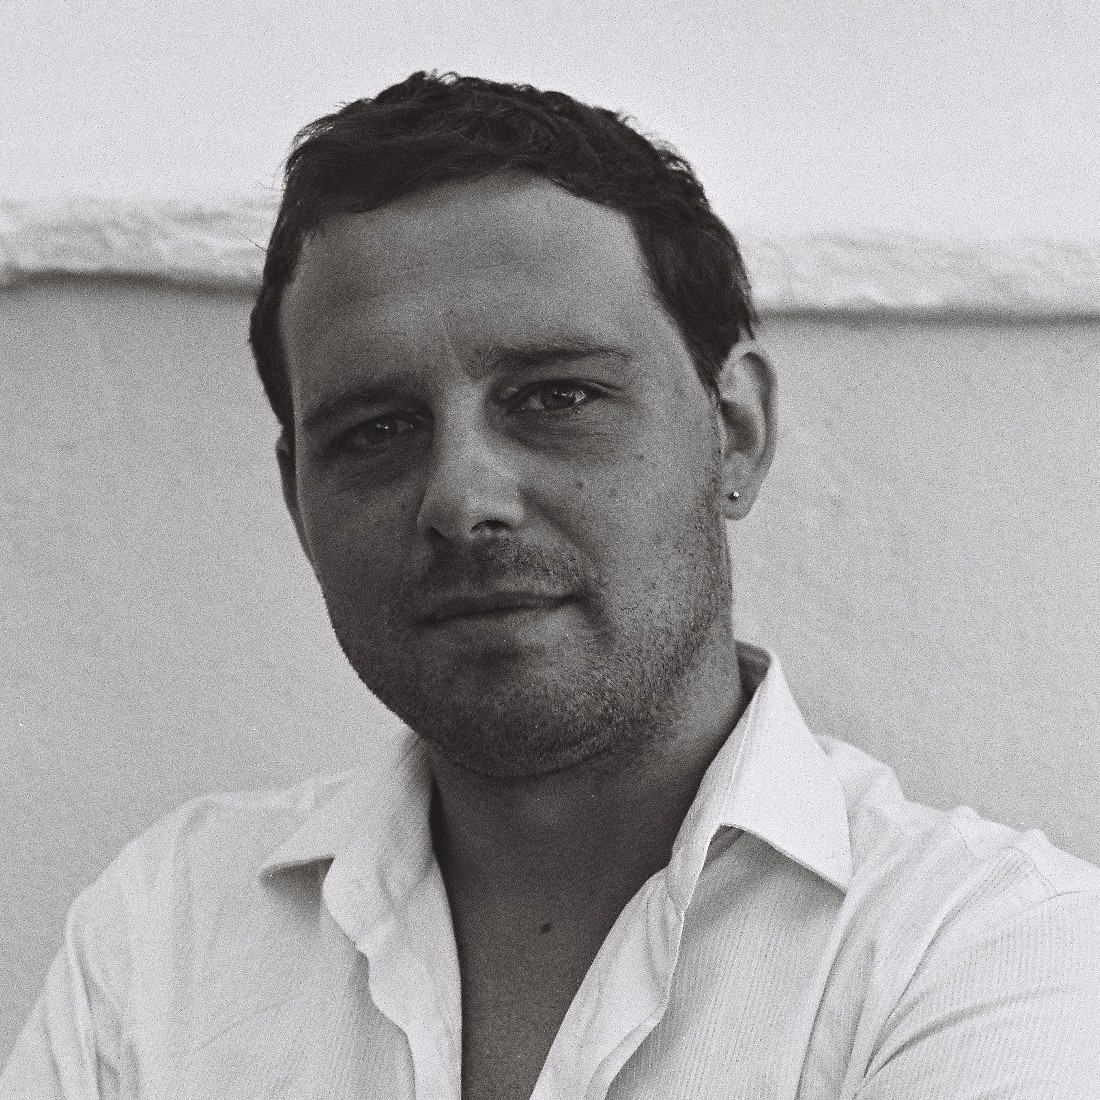
\includegraphics[width=\linewidth]{ja-mali.jpg} &

    \renewcommand{\arraystretch}{2.5}
    \begin{tabular}{@{}|l}

      \textsc{\huge{Drasko Draskovic}} \\
      \large{R\&D Engineer and Software Architect} \\

      \renewcommand{\arraystretch}{1}
      \begin{tabular}{@{}lll}
        \small{\faAt} drasko.draskovic@gmail.com &
        \small{\faEnvelopeO} 135 Rue D'Alesia, 75014 &
        \small{\faMapMarker} Paris, France \\
        \small{\faLinkedin} \href{https://www.linkedin.com/in/draskodraskovic}{@draskodraskovic} &
        \small{\faGithub} \href{https://github.com/drasko}{@drasko} &
        \small{\faTwitter} \href{https://twitter.com/draskodraskovic}{@draskodraskovic}
      \end{tabular}

    \end{tabular}

  \end{tabular}

\vspace{6mm}

\begin{minipage}[t]{0.48\linewidth}
  \section{Work Experience}

  \vspace{3mm}

  %%%%%%
  %% Nokia
  %%%%%%
  {\color{Gray}
    \begin{tabular*}{\linewidth}{@{}l@{\extracolsep{\fill}}l}
      {\color{RubineRed} \textsc{Nokia}} \smallskip & \\
      \small{\faCalendar} \hspace{0.01\linewidth} November 2014 -- Present & \small{\faMapMarker} \hspace{0.01\linewidth} Paris, France \\
    \end{tabular*}

    \smallskip
    {\color{Black}\textbf{Senior R\&D Engineer and Software Architect}}
  }

  \begin{itemize}
    \item Obtained grant from internal Nokia internal Venture Capital
          accelarator to bootstrap new bussiness around Blockchain technology:
      \begin{itemize}
        \item Architectured and implemented (from scratch) IoT data monetization platform based on Hyperledger Fabric blockchain,
            with internal cryptocurrency Smart Contract and complete security and deployment infrastructure
        \item Invented and filed a patent on mechanism for temporary data stream access via blockchain-configured decentralized proxy
        \item Managed a team of 4 developers
        \item Designed start-up finance and marketing plans and managed relations with investors and various stakeholders
        \item Led two big international pilot projects for blockchain product with telecom operators from Europe and Middle East
      \end{itemize}
    \item Implemented (in C++) 5G features for new Nokia projects
    \item Assured Quallcom deliveries of Linux BSP for multi-standard LTE femto-cells on projects for AT\&T and T-Mobile
  \end{itemize}

  %%{\color{Gray} \hdashrule{\linewidth}{0.3pt}{4pt}}

  \vspace{3mm}

  %%%%%%
  %% Devialet
  %%%%%%
  {\color{Gray}
    \begin{tabular*}{\linewidth}{@{}l@{\extracolsep{\fill}}l}
      {\color{RubineRed} \textsc{Devialet}} \smallskip & \\
      \small{\faCalendar} \hspace{0.01\linewidth} March 2013 -- November 2014 & \small{\faMapMarker} \hspace{0.01\linewidth} Paris, France \\
    \end{tabular*}

    \smallskip
    {\color{Black}\textbf{Software Architect}}
  }

  \medskip

  Work on system design and embedded SW architecture
  of wireless digital audio system based on dual-core
  ARM Cortex-A9 FPGA with custom hard-RT Xenomai-patched
	Yocto Linux kernel and dual-band 802.11abgn WiFi connection.

  \vspace{7mm}

  %%%%%%
  %% Sequans
  %%%%%%
  {\color{Gray}
    \begin{tabular*}{\linewidth}{@{}l@{\extracolsep{\fill}}l}
      {\color{RubineRed} \textsc{Sequans Communications}} \smallskip & \\
      \small{\faCalendar} \hspace{0.01\linewidth} June 2010 -- March 2013 & \small{\faMapMarker} \hspace{0.01\linewidth} Paris, France \\
    \end{tabular*}

    \smallskip
    {\color{Black}\textbf{Embedded Platform Engineer}}
  }

  \medskip

  Work on platform enablement, system and device drivers for LTE
  multi-processor SoCs, based on ARM and MIPS architectures
  with eCos RTOS (for baseband CPU) and Linux (for application CPU).

  \vspace{7mm}

  %%%%%%
  %% Elsys
  %%%%%%
  {\color{Gray}
    \begin{tabular*}{\linewidth}{@{}l@{\extracolsep{\fill}}l}
      {\color{RubineRed} \textsc{Elsys Design}} \smallskip & \\
      \small{\faCalendar} \hspace{0.01\linewidth} June 2006 -- June 2010 & \small{\faMapMarker} \hspace{0.01\linewidth} Paris, France \\
    \end{tabular*}

    \smallskip
    {\color{Black}\textbf{Software Engineer}}
  }

  \medskip

  Consulting work in SW engineering for various clients:
  \textbf{Philips} (Set-Top Box for \textit{Canal+}),
  \textbf{Spidcom} (Linux kernel and device drivers for ARM-based PLC SoC) and
  \textbf{Texas Instruments} (OMAP platform development)

  \medskip

  %%%%%%
  %% Education
  %%%%%%
  \section{Education}

    \textbf{\textsc{Diploma Engineer (equivalent to M.Sc.)}} \\
    School of Electrical Engineering, University of Belgrade,
    department of Electronics, Telecommunications and Control

    \medskip

    \textbf{Master Thesis in Audiotechnics} : \textit{"Analysis of Methods And
         Applications for Artificial Reverberation"}

\end{minipage}\hspace{0.04\linewidth}
\begin{minipage}[t]{0.45\linewidth}

  \fcolorbox{Lavender}{Lavender}{
    \begin{minipage}[t]{0.95\linewidth}

      \section{Technical Skills}

      \textbf{IoT} and \textbf{Blockchain} expert with entrepreneurial spirit and over 10 years of professional experience in:

      \bigskip

      \setlength{\arrayrulewidth}{0.5mm}
      \renewcommand{\tabularxcolumn}[1]{>{\arraybackslash}m{#1}}

      \begin{tabularx}{\linewidth}{m{0.12\linewidth}|X}
        Arch & Scalable distributed systems,
            decentralized computing and p2p messaging,
            edge computing, message buses,
            microservices, 5G, security, API design,
            logging \& instrumenting, domain-driven design, cloud-native, twelve-factor apps
      \end{tabularx}

      \medskip

      \begin{tabularx}{\linewidth}{m{0.12\linewidth}|X}
        HW & Linux kernel and device drivers, RTOSes, bootloaders,
          JTAG debugging, communication protocols (WiFi, BLE, 6LoWPAN, LoRaWAN),
          HW interfaces (I$^2$C, SPI, UART, USB), FPGA \& PCB design
      \end{tabularx}

      \medskip

      \begin{tabularx}{\linewidth}{m{0.12\linewidth}|X}
        SW & C/C++, Go, Python, Erlang/OTP, Elixir, NodeJS, Lua, Rust, Bash, Perl, Nim
      \end{tabularx}

      \medskip

      \begin{tabularx}{\linewidth}{m{0.12\linewidth}|X}
        DevOps & Docker, Kubernetes, Ansible, CI, Load Balancers, Reverse Proxies
      \end{tabularx}
    \end{minipage}
  }

  \medskip

  \section{Open-Source Projects}
    GNU and FOSS evangelist, implicated in many open source projects in domains of
    architecture, development, maintaining, documentation and support.

    \begin{itemize}
      \item \href{https://www.edgexfoundry.org}{EdgeX Foundry} by Linux Foundation -- maintainer
      \item \href{https://github.com/Mainflux/mainflux}{Mainflux} IoT Platform -- author and main architect
      \item \href{http://www.we-io.net}{WeIO} IoT Board -- author and main architect
    \end{itemize}

  \section{Publications \& IP}
    \faBook \hspace{1mm} \textsc{Books}
    \begin{itemize}
      \item  Ervin Varga, Drasko Draskovic and Dejan Mijic, \href{http://www.oreilly.com/programming/free/scalable-architecture-for-the-internet-of-things.csp}
        {\textit{"Scalable Architecture for the Internet of Things"}},  O'Reilly Media, 2018.
    \end{itemize}

    \medskip

    \faFileTextO \hspace{1mm} \textsc{Patents}
    \begin{itemize}
      \item Drasko Draskovic and George Saleh, \textit{"Mechanism and Aparatus for Selling Data Streams via Blockchain with Temporary Proxied Access"},
        PAN 18305283.6, Nokia, 2018.
    \end{itemize}

    \medskip

    \faTrophy \hspace{1mm} \textsc{Awards}
    \begin{itemize}
      \item Innovation Award - \href{https://www.edgexfoundry.org/blog/2018/04/24/happy-1st-anniversary-edgex-foundry}{Linux Foundation's EdgeX Foundry Community Awards 2018}
      \item Contribution Award - \href{https://www.edgexfoundry.org/blog/2018/04/24/happy-1st-anniversary-edgex-foundry}{Linux Foundation's EdgeX Foundry Community Awards 2018}
    \end{itemize}

    \medskip

    \faGroup \hspace{1mm} \textsc{Conferences}
    \begin{itemize}
      \item Open IoT Summit, \href{http://sched.co/DYM7}{\textit{"Hyperscalable Unified IoT Architecture"}}, Linux Foundation, Portland, USA, 2018
      \item Software Architecture Conference, \href{https://conferences.oreilly.com/software-architecture/sa-eu-2017/public/schedule/detail/62113}
        {\textit{"Architecturing and Securing IoT Platforms with Microservices"}}, O'Reilly, London, UK, 2017
      \item Open Networking Summit, \href{http://sched.co/9x8L}{\textit{"IoT and Networking -- Architecture, Requirements \& Implementation"}}, Linux Foundation, Santa Clara, USA, 2017
    \end{itemize}

    \section{Communication Skills}
      \textbf{English} (excellent), \textbf{French} (excellent), \textbf{Russian} (understanding), \textbf{Serbian} (mother tongue)

\end{minipage}
\end{document}
